%! Author = idegen
%! Date = 26/11/2021

\documentclass[a4paper]{article}
\usepackage[margin=1in]{geometry}
\usepackage[dvipsnames]{xcolor}
\usepackage[utf8]{inputenc}
\usepackage[english]{babel}
\usepackage[default,oldstyle,scale=0.95]{opensans}
\usepackage[]{amsthm}
\usepackage[]{amssymb}
\usepackage{placeins}
\usepackage{textcomp}
\usepackage{setspace}
\usepackage{fancyhdr}
\usepackage[useregional]{datetime2}
\usepackage{hyperref}
\hypersetup{
    colorlinks=true,
    linkcolor=Emerald,
    filecolor=magenta,
    urlcolor=cyan,
    citecolor=RoyalBlue
}
\usepackage{graphicx}
\usepackage{caption}
\usepackage{subcaption}
\graphicspath{ {./images/} }
\usepackage{textcomp}
\usepackage{outlines}
\usepackage{tabularx}
\usepackage[T1]{fontenc}
\usepackage{scrextend}
\usepackage{multirow}
\makeatletter
\def\namedlabel#1#2{\begingroup
#2%
\def\@currentlabel{#2}%
\phantomsection\label{#1}\endgroup
}
\makeatother

\setlength{\parindent}{0em}
\setlength{\parskip}{0.5em}

\pagestyle{fancy}
\fancyhf{}
\chead{Machine Learning Paradigms}
\rhead{\today}
\lhead{Isabella Degen}
\lfoot{isabella.degen@bristol.ac.uk}
\rfoot{Page \thepage}

\title{Machine Learning Paradigms - Coursework Report}
\author{Isabella Degen - Interactive AI CDT}

\begin{document}
    \maketitle


    \section{Introduction and Approach}\label{sec:introduction}
    My goal for this coursework was to gain more experience with a few ML algorithms, evaluation methods and
    different Python frameworks available. I was also keen to use experiment tracking methods, as
    well as further improve my software engineering practices when writing an ML system. I was less focused on
    finding the best solution for the problem.

    I followed the steps on \href{https://www.kaggle.com/c/morebikes2021/overview/description}{Kaggle}. I wrote a solution
    for both approaches:
    \begin{itemize}
        \item[(a)] separate model for each station
        \item[(b)] single model for all stations together
    \end{itemize}

    The way I setup my scripts made it a simple change of configuration to train a model for all stations or one model
    or either one of them using any ML algorithm.

    I further broke down the work for each of these two approaches into the following steps:
    \subsection*{\label{phs:one}{Phase 1}}
    Predict the availability of bikes for stations 201-275
    \begin{description}
        \item [\namedlabel{itm:phase1-step1}{Step 1.1}] Analyse and investigate the data and decide what ML problem it is
        \item [\namedlabel{itm:phase1-step2}{Step 1.2}] Create an end to end pipeline with a simple model for approach a) and b)
        \item [\namedlabel{itm:phase1-step3}{Step 1.3}] Feature engineering and experiment more with different models
        \item [\namedlabel{itm:phase1-step4}{Step 1.4}] Tune promising setups
    \end{description}

    I submitted models to Kaggle before I did the tuning as I wanted to make sure I got the format right and wanted to
    gain insights on how well my models were performing on the test data.

    \subsection*{\label{phs:two}{Phase 2}}
    Use the pre-trained models for station 1-200 to predict the availability of bikes for stations 201-275
    \begin{description}
        \item [\namedlabel{itm:phase2-step1}{Step 2.1}] Analyse the given models
        \item [\namedlabel{itm:phase2-step2}{Step 2.2}] Create an end to end pipeline for the given models
        \item [\namedlabel{itm:phase2-step3}{Step 2.3}] Investigate the resulting performance and compare to \nameref{phs:one}
    \end{description}

    \subsection*{\label{phs:three}{Phase 3}}
    Combine the approaches from \nameref{phs:one} and \nameref{phs:two}
    \begin{description}
        \item [\namedlabel{itm:phase3-step1}{Step 3.1}] Create an end to end pipeline for the combining the models from \nameref{phs:one} and \nameref{phs:two}
        \item [\namedlabel{itm:phase3-step2}{Step 3.2}] Tune promising setups
        \item [\namedlabel{itm:phase3-step3}{Step 3.3}] Investigate the resulting performance and compare to \nameref{phs:one} and \nameref{phs:two}
    \end{description}

    I keep referring back to these steps in the sections \nameref{sec:technical-background}, \nameref{sec:method}, \nameref{sec:experiment-setup} and
    \nameref{sec:results}. The \nameref{sec:conclusions} sections gives a summary of my overall learnings and conclusions.

    The code for this coursework is available from my GitHub \href{https://github.com/isabelladegen/mlp-2021}{mlp-2021} repository and
    all of the tracked runs are available on my \href{https://wandb.ai/idegen/mlp-2021}{Weights \& Biases - MLP 2021 workspace}.


    \section{Technical Background}\label{sec:technical-background}

    While I wrote my Dialogue and Narrative coursework, I made the painful experience on how quickly a
    simple ML system can get messy. It's
    easy to spend endless time analysing the data in Jupyter Notebooks, running a few experiments, seeing promising results,
    forgetting what the exact setup for those were and then never be able to reproduce them again. Learning from this
    experience I decided to do use hopefully better engineering practices for this coursework. This meant
    that I decided to write all the experiments that went beyond poking around in the data in pure Python. I used test
    driven development to implement the scripts and classes. While the tests are not exhaustive they are touching every
    part of the module and allowed me to find countless mistakes I inevitably made. They also serve as a nice and living
    documentation how to use the different classes and scripts.

    To keep track of the configuration and results for different experiments I used the
    \href{https://wandb.ai/site}{Weights \& Biases platform}\cite{wandb}.
    I shall refer to the Weights \& Biases platform from now on by its Python package name \textit{wandb}. To make full
    use of wandb's capabilities to track experiments I made sure that all hyper parameters,
    conditional processing logic and other magical numbers and strings in the codebase were kept in a configuration
    dataclass that was logged as \texttt{wandb.config}. While initially the purpose for the configuration's dataclass was for experiment
    tracking, it also enabled me to quickly change the setup, run sweeps to tune hyper parameters and other model setups.

    I created a mlp-2021 conda environment on my mac \cite{conda-forge} which can be built and updated using the
    \href{https://github.com/isabelladegen/mlp-2021/blob/main/conda.yml}{conda.yml} file. I only fix the version of Python to 3.9,
    for the other libraries I want to use their newest version. Wandb automatically produces a \texttt{requirements.txt}
    as well as a \texttt{environment.yml} file for each run which lists the exact version of all the libaries an their
    dependencies. This should allow to recreate the exact Python setup used while also making it easy to keep working with
    the newest version unless their should be a reason to fix to a specific version, which I've not come accross for this coursework.

    The \href{https://github.com/isabelladegen/mlp-2021}{Readme} on Github describes how to setup the environment as well
    as how to run the various experiments which can also be seen on on my \href{https://wandb.ai/idegen/mlp-2021}{Wandb - MLP 2021 workspace}.

    Given I was working with simple ML algorithms, I ran all the experiments on my personal laptop.


    \section{Method}\label{sec:method}

    In this section I describe the method used for each of the steps listed in the \nameref{sec:introduction}.

    \subsection*{\nameref{phs:one}}

    For this coursework we were given a dataset for stations 201-275 with 744 labelled samples per station
    resulting in a total 55800 labelled samples. While we were also given a test dataset, the test dataset had no labels
    and therefore could not be used to validate my models during development of the system. For that reason I randomly
    took 10\% of samples away from the 55800 labelled samples. I call the resulting dataset of 5580 labelled data the validation
    dataset and the remaining dataset of 50220 labelled samples the training or dev dataset. All the models are only
    trained on the training dataset. This setup allowed me to verifiy my models performance on unseen data.

    \subsubsection*{\nameref{itm:phase1-step1}}
    The goal for this step is to gain a better idea of what sort of problem we've been given. For this I looked at the
    given dataset on a very high level. I wanted to know how much data we were given, what type of data we were given and
    generally understand
    a bit more what the data means. As I moved to \nameref{itm:phase1-step2} I continued to come back to this step
    to understand more about how many data points were nan to decide how to best pre-process the data for a new column.


    \subsubsection*{\nameref{itm:phase1-step2}}
    As described in \nameref{sec:conclusions} I create a \textit{pipeline} setup where I didn't needed to decide
    on an algorithm and that let me easily experiment and evaluate different models, features and ways of data processing.

    I also wanted to create a baseline. For this I wrote a random estimator that returns a random number of bikes between
    0 and the number of docks for the station.

    Following from that, I created a model for all stations as well as a model per station using the PoissonRegressor from
    scikit-learn \cite{scikit-learn}. The difference between approach a) and b) was a simpler wrapper class that split the
    overall dataframe of all stations back into the data per station and that managed the multiple models. The results
    two can both deal with per station results, overall results and report on per station mean absolut error or
    overall absolute error.

    For both I used bikes\_3h\_ago as feature matrix X. Given 300 rows are missing this value I had to decide what to do
    with a nan value. Possibilities I thought of were: just drop those samples, use the mean number of bikes. I didn't wanted
    to drop 300 samples as I was invevitably going to drop a lot more samples with that strategy when adding more features.
    I decided to put the nan values to the most frequent value. For the per station data that meant to the most frequent for
    the station, for the one model for all stations that meant to the most frequent value overall.

    Given I wanted to make it super easy to swap models and given the results were not great for the PoissonRegressor
    I also added a RandomForestRegressor model from scikit-learn. This made me pull the code out of the PoissonModel class
    into an \texttt{abstract} Model class that is doing the \texttt{fit()} and \texttt{predict()} and creating a result.
    The only bit of code needed for a specific model was the configuration of that model. I reused the same run script
    by passing it the name of the class instead of an instance, so it could create the model itself depending on its configuration.

    For unit testing of the code I used fake data setup in builder classes as well as a smaller data subset of real data.

    I ran a wandb experiment for all of these three naive models: random guessing, poisson regressor and random forest
    regressor with just one feature.

    \subsubsection*{\nameref{itm:phase1-step3}}
    At this point I wanted to include more features into the training to see if I could reduce the prediction error
    especially for the stations that are performing much worse than others. I was still continuing to test both approaches:
    a model per station as well as one model for all stations. However I decided to work with the RandomForestRegressor
    as it was performing better than the PoissonRegressor. I also decided to play with features that I could understand
    what they meant and so I left out the bike profile features (which in hindsight was a mistake).

    Features I wanted to investigate were:
    \begin{itemize}
        \item \textbf{Weather Data}: I'm assuming this is similar across the different stations but could have an impact on
        if people are using more or less motorbikes.
        \item \textbf{Station Data}: For the one model for all station approach it could be beneficial to including station specific data such as longitude
        and latitude, number of docks - bigger stations might be at busier locations than smaller stations, or even just the station id.
        \item \textbf{Situational data}: Weekhour could help help with changes in demand for different times of the day and different days of the week.
        Similarly isHoliday could perhaps help to distinguish between times that have very different demands.
        \item \textbf{}
        \item \textbf{}
        \item \textbf{}
    \end{itemize}

    For each features I needed to decide what pre-processing steps were needed and if and how I could sensibly fill the nan values
    for the feature.

    \subsubsection*{\nameref{itm:phase1-step4}}
    Use weight and biases sweep ability. Define a few different hyperparameters, make a smaller data set (runtime!) and
    sweep through the parameters to learn which ones have what effect. Iterate multiple times with what works and
    see if the results from the default configuration can be imporved.

    \subsection*{\nameref{phs:two}}
    \subsubsection*{\nameref{itm:phase2-step1}} Analyse the given models
    \subsubsection*{\nameref{itm:phase2-step2}} Create an end to end pipeline for the given models
    \subsubsection*{\nameref{itm:phase2-step3}} Investigate the resulting performance and compare to \nameref{phs:one}

    \subsection*{\nameref{phs:three}}
    \subsubsection*{\nameref{itm:phase3-step1}} Create an end to end pipeline for the combining the models from \nameref{phs:one} and \nameref{phs:two}
    \subsubsection*{\nameref{itm:phase3-step2}} Tune promising setups
    \subsubsection*{\nameref{itm:phase3-step3}} Investigate the resulting performance and compare to \nameref{phs:one} and \nameref{phs:two}

%%%%%%%%%%%%%%%%%%%%%%%%%%%%%%%%%%%%%%%%%%%%%%


    \section{Experiment Setup}\label{sec:experiment-setup}
    I'm using the JetBrains DataSpell IDE for working with Notebooks and PyCharm IDE for working with Python. Both IDEs offer
    a rich debugging and runtime environment, test and script execution and advanced refactoring abilities.

    \subsection*{\nameref{phs:one}}

    \subsubsection*{\nameref{itm:phase1-step1}}
    I mostly used the
    \href{https://github.com/isabelladegen/mlp-2021/blob/main/notebooks/ExperimentWithPerStationData.ipynb}{ExperimentWithPerStationData.ipynb}
    Jupyter notebook and loaded the data into a pandas dataframe \cite{reback2020pandas} which overs various methods
    to get a quick insights of the data such as: \texttt{info()}, \texttt{describe()} and \texttt{value\_counts()} as well
    as methods to count nan's.

    \subsubsection*{\nameref{itm:phase1-step2}}
    All the code for the pipeline is just pure Python and can be found in the
    \href{https://github.com/isabelladegen/mlp-2021/tree/main/src}{src} folder on GitHub. There are two
    scripts to run either the random estimator or a model based estimator:
    \begin{enumerate}
        \item \href{https://github.com/isabelladegen/mlp-2021/blob/main/src/random_predictions.py}{random\_predictions.py}:
        It uses the \href{https://github.com/isabelladegen/mlp-2021/blob/c48d85dc364b5a2e7e59f16961b32f9e6c245735/src/models/RandomEstimator.py}{RandomEstimator}
        class to estimate a random number of bikes
        \item \href{https://github.com/isabelladegen/mlp-2021/blob/main/src/simple_regression.py}{simple\_regression.py}: It creates
        an instance of the \href{https://github.com/isabelladegen/mlp-2021/blob/main/src/models/Model.py}{Model} class given, which
        can be either for this experiment was either the \href{https://github.com/isabelladegen/mlp-2021/blob/main/src/models/PoissonModel.py}{PoissonModel}
        or the \href{https://github.com/isabelladegen/mlp-2021/blob/main/src/models/RandomForestRegressorModel.py}{RandomForestRegressorModel}.
    \end{enumerate}

    Each model implements \texttt{predict()} which returns a  \href{https://github.com/isabelladegen/mlp-2021/blob/c48d85dc364b5a2e7e59f16961b32f9e6c245735/src/PredictionResult.py}{PredictionResult}
    class that is used for evaluation of the model. It calculates the overall mean absolute error (MAE) using \texttt{mean\_absolute\_error}
    from scikit-learn, as well as the the MAE for each station. Furthermore the result also implements the
    \texttt{write\_to\_csv()} function that writes the predictions to a csv file using the format required for the Kaggle submissions.

    The \texttt{run} script calls \texttt{wandb.init(...)} to start the experiment tracking, loads the training data using the required data,
    creates both a single model and a model per station depending on the configuration, trains the model calling \texttt{fit()},
    predicts the number of bikes for the training, validation and test data sets calling the different models \texttt{predict(...)}
    functions which each return a prediction result, which is then called to log the overall MAE as well as the per
    station MAE for the training and validation dataset, this is logged to wanddb using \texttt{wandb.log(...)} and finally
    the script creates a csv for a Kaggle submission. All the rest of the experiment is automatically tracked by wandb
    and the results can be visualised on there.

    The \href{https://github.com/isabelladegen/mlp-2021/blob/c48d85dc364b5a2e7e59f16961b32f9e6c245735/src/Data.py}{Data} class
    is used to load all the data and also does all of the pre-processing based on configuration values. It encapsulates
    a pandas dataframe and provides easy access function to get the feature matrix X and the labelled data y. It's further
    capable of operating on all data or of returning a Data class for each station. The Data class is loading the
    bikes\_3h\_ago column as pandas \texttt{category} type and is using the
    \texttt{SimpleImputer(strategy="most\_frequent")} from scikit-learn to fill the nan values for bikes\_3h\_ago.

    Finally all the configurations are stored in the Configurations dataclass defined in
    \href{https://github.com/isabelladegen/mlp-2021/blob/c48d85dc364b5a2e7e59f16961b32f9e6c245735/src/configurations.py}{configurations.py}.
    This script also provides a TestConfiguration class that disables the upload to wandb for unit testing purposes but
    still ensures the calls are syntactically correct. At this stage both the PoissonRegressor as well as the RandomForestRegressor
    were using their default configurations. However,
    I've already made these hyper parameters configurable so that they automatically get logged in wandb.

    Finally, I wrote a helper \href{https://github.com/isabelladegen/mlp-2021/blob/c48d85dc364b5a2e7e59f16961b32f9e6c245735/src/create_dev_and_validation_csv.py}{script}
    to create the training and validation dataset and write them as .csv files in my local
    data folder. Each experiment is using the same training and validation datasets, loading them from these .csv files.

    The code as evolved since this experiment, the hashes listed below can be used to get the versions at the time of
    these first simple experiment runs:

    \begin{itemize}
        \item \textbf{Random Prediction}: \\git checkout -b "classic-sun-10"\footnote{\label{fn:wand-db-name}wandb run name} c22db5e7b461cfd7ba7e7af81460d93b984b2e14
        \item \textbf{Poisson Regressor}: \\git checkout -b "chocolate-serenity-19"\footref{fn:wand-db-name} e1c7158a2f41568b7781d00cc0d5330982edc398
        \item \textbf{Random Forest Regressor}: \\git checkout -b "peach-bird-23"\footref{fn:wand-db-name} e6e86614d7e62a3f09bd635c8125f479c0d4e971
    \end{itemize}

    \subsubsection*{\nameref{itm:phase1-step3}}
    The underlying infrastructure was in place by from the previous step. All I needed to do is change the configurations
    and decide what to do with the nan values. I used the
    \href{https://github.com/isabelladegen/mlp-2021/blob/c48d85dc364b5a2e7e59f16961b32f9e6c245735/notebooks/TestAndTrainingDataForFeatureSelection.ipynb}{TestAndTrainingDataForFeatureSelection.ipynb}
    Jupyter notebook to find get some high level statistics about the features I was about to add. I decided early
    on (and mistakenly) not to include the bike profile features due to the many nan values. The location feature investigation is
    in the \href{https://github.com/isabelladegen/mlp-2021/blob/c48d85dc364b5a2e7e59f16961b32f9e6c245735/notebooks/InvestigateFeatures.ipynb}{InvestigateFeatures.ipynb}
    Jupyter notebook.

    I mostly used the RandomForestRegressor for this investigation. Table \ref{tbl:feature-exploration-overview} gives an
    overview of the different
    features explored as well as a link to the wandb logs for each of the relevant run. While analysing the
    weather data I noticed that precipitation had no training data at all and was therefore not going to be useful for training and
    the ranges of temperature between the training and the test dataset did not overlap well so I decided to leave that out
    for now too.

    \begin{table}[h]
        \centering
        \begin{tabularx}{\textwidth}{|X|X|X|X|}
            \hline
            \textbf{Feature (s)}                                                    & \textbf{\#nan}                                                  & \textbf{Type} & \textbf{Experiment Id}                                                                                            \\ \hline
            numDocks                                                                & no nan                                                          & category      & \href{https://wandb.ai/idegen/mlp-2021/runs/185f8iiz?workspace=user-idegen}{autumn-rain-25}    \\ \hline
            station                                                                 & no nan                                                          & category      & \href{https://wandb.ai/idegen/mlp-2021/runs/3ikbmzvm?workspace=user-idegen}{wobbly-hill-29}    \\ \hline
            weekhour                                                                & no nan                                                          & category      & \href{https://wandb.ai/idegen/mlp-2021/runs/36vs3wjd?workspace=user-idegen}{easy-capybara-30}  \\ \hline
            windMeanSpeed.m.s, windDirection.grades, relHumidity.HR, airPressure.mb & all each had the same 75 samples with nan, fill with mean value & float         & \href{https://wandb.ai/idegen/mlp-2021/runs/2ncnkrj2?workspace=user-idegen}{vital-hill-32}     \\ \hline
            isHoliday                                                               & 75 nan, fill with most frequent value                           & category      & \href{https://wandb.ai/idegen/mlp-2021/runs/140v0dji?workspace=user-idegen}{astral-feather-33} \\ \hline
        \end{tabularx}
        \caption{Overview of features explored, strategy for how to fill nan and link to the experiment on wanddb.}
        \label{tbl:feature-exploration-overview}
    \end{table}



    \subsubsection*{\nameref{itm:phase1-step4}}

    1. Sweep just with a few hyper parameters and 10\% of the dev and val data (dev-sweep1, val-sweep1).
    - Only sweep one model as it's quicker
    - Results of sweep in Random Forest Sweep 1 https://wandb.ai/idegen/mlp-2021/sweeps/ylvvcigm?workspace=user-idegen
    - method: grid
    name: Random forest sweep 1
    parameters:
    random\_forest\_bootstrap:
    values:
    - false
    random\_forest\_ccp\_alpha:
    values:
    - 0
    - 0.05
    - 0.1
    - 0.3
    random\_forest\_criterion:
    values:
    - squared\_error
    - poisson
    random\_forest\_max\_depth:
    values:
    - null
    - 10
    - 50
    random\_forest\_min\_samples\_split:
    values:
    - 2
    - 4
    random\_forest\_n\_estimators:
    values:
    - 50
    - 100
    - 120
    -> For the best sweep result re-run the full model:
    Silver Plasma: https://wandb.ai/idegen/mlp-2021/runs/1t2bcd2d/overview?workspace=user-idegen
    -> Best sweep result
    Features:
    ["station","bikes\_3h\_ago","numDocks","weekhour","isHoliday","full\_profile\_bikes","full\_profile\_3h\_diff\_bikes"]
    Differnce in hyperparams:
    random\_forest\_max\_depth: 50
    random\_forest\_n\_estimators: 50
    random\_forest\_ccp\_alpha: 0.05
    random\_forest\_criterion: squared\_error

    Breezy Sound: https://wandb.ai/idegen/mlp-2021/runs/12p54n9c/overview?workspace=user-idegen
    -> New parameters but features as current best run with default configuration
    Features: ["station","bikes\_3h\_ago","numDocks","weekhour","isHoliday"]
    random\_forest\_max\_depth: 50
    random\_forest\_n\_estimators: 50
    random\_forest\_ccp\_alpha - 0.05
    random\_forest\_criterion: squared\_error

    Stoic Sun: https://wandb.ai/idegen/mlp-2021/runs/12zlftk6/overview?workspace=user-idegen
    -> Features from best run squared error and ccp from sweep, max depth and n estimator from best run
    random\_forest\_features
    Features: ["station","bikes\_3h\_ago","numDocks","weekhour","isHoliday"]
    random\_forest\_max\_depth: Default
    random\_forest\_n\_estimators: 100
    random\_forest\_ccp\_alpha - 0.05
    random\_forest\_criterion: squared\_error

    Sweep 2: https://wandb.ai/idegen/mlp-2021/sweeps/79bi8rgn/overview
    - 30\% of training data
    - Model per station
    - Different features, ccp
    -> lead to an improval on astral feather with zesty field

    Sweep 3:
    - try some other pruning methods

    Sweep 4: Features and Hyperparmetes including feature combination used in the given models
    - use full data for sweeping as runtime is low at the momemnt


    \subsection*{\nameref{phs:two}}
    \subsubsection*{\nameref{itm:phase2-step1}} Analyse the given models
    \subsubsection*{\nameref{itm:phase2-step2}} Create an end to end pipeline for the given models
    \subsubsection*{\nameref{itm:phase2-step3}} Investigate the resulting performance and compare to \nameref{phs:one}

    \subsection*{\nameref{phs:three}}
    \subsubsection*{\nameref{itm:phase3-step1}} Create an end to end pipeline for the combining the models from \nameref{phs:one} and \nameref{phs:two}
    \subsubsection*{\nameref{itm:phase3-step2}} Tune promising setups
    \subsubsection*{\nameref{itm:phase3-step3}} Investigate the resulting performance and compare to \nameref{phs:one} and \nameref{phs:two}

%%%%%%%%%%%%%%%%%%%%%%%%%%%%%%%%%%%%%%%%%%%


    \section{Results}\label{sec:results}
    Results achieved

    \subsection*{\nameref{phs:one}}
    Overall:

    \subsubsection*{\nameref{itm:phase1-step1}}
    The dataset we are given has 55875 samples. 75, exactly one per station, of these samples are missing their label ('bikes'
    column value null).
    I decided to simply exclude those rows, meaning I had in total 55800 labelled samples, 744 per station. Furthermore,
    13275 rows have a least one nan value in other columns.
    We've been given various information:
    \begin{itemize}
        \item \textbf{Information about the station}: tation (station id), latitude, longitude and
        numDocks (number of available bike docks)
        \item \textbf{Information about the time when the sample was taken}: timestamp, year, month, day, hour,
        weekday, weekhour (a combination of weekday and hour), isHoliday (marking public holidays)
        \item \textbf{Information about the weather}: windMaxSpeed.m.s, windMeanSpeed.m.s,  windDirection.grades,
        temperature.C, relHumidity.HR, airPressure.mb, precipitation.l.m2
        \item \textbf{Information about the bike usage}: bikes\_3h\_ago, full\_profile\_3h\_diff\_bikes,
        full\_profile\_bikes, short\_profile\_3h\_diff\_bikes, short\_profile\_bikes, bikes
    \end{itemize}

    Other than the information about the bike usage, these all made sense. I'm to this day not sure what the columns
    about the bike usage actually mean other than bikes\_3h\_ago persumably is the number of bikes at the station 3h
    before the sample was taken and bikes is the number of bikes at the station when the sample was taken. Curiously it
    is possible for a station to have and record more bikes than the number of docks available.

    Not all data types are useful in their raw format. E.g weekday would need to be translated into a numerical value.
    Other than the weather data the given data was categorical.

    \subsubsection*{\nameref{itm:phase1-step2}}

    I ran multiple experiments for Random Guessing, basic Poisson Regressor and Random Forest Regressor, however
    representative runs on wandb are listed below as reference for the results and configurations used, further runs can
    be found e.g using tags:
    \begin{itemize}
        \item \href{https://wandb.ai/idegen/mlp-2021/runs/3k64fgcw/overview?workspace=user-idegen}{Random Guessing} - classic-sun-10
        \item \href{https://wandb.ai/idegen/mlp-2021/runs/1iyx8zmh/overview?workspace=user-idegen}{Poisson Regressor} - chocolate-serenity-19
        \item \href{https://wandb.ai/idegen/mlp-2021/runs/25zvoihx/overview?workspace=user-idegen}{Random Forest Regressor} -peach-bird-23
    \end{itemize}

    Table \ref{tbl:phase1-step2-simple-model-mae} shows that random guessing is in average 7 bikes off, while both ML models
    outperformed random guessing and were only around 3 bikes off. The random forest regressor performed slightly better and
    for both ML models the model per station peformed better than a single model for all stations. All models
    were reasonable quick to train and run: random guessing took 8s, 1m 55s and the Random Forest Regressor took 11m 7s.
    These timings are to be taken with a pinch of salt as the experiment was run on my machine with many other applications
    running at the same time. They can only be used to get a general feeling. If of interest, wandb does
    also log CPU, memory and disk utilisation. For the two ML models the time includes both training of the single model
    as well as training of a model per station.

    \begin{table}[h]
        \centering
        \begin{tabularx}{\textwidth}{|X|XX|XX|XX|}
            \hline
            \multirow{2}{*}{MAE} & \multicolumn{1}{l|}{Random Guessing} & & \multicolumn{2}{l|}{Poisson Regressor} & \multicolumn{2}{l|}{Random Forest Regressor} \\ \cline{2-7}
            & \multicolumn{1}{l|}{Training} & Validation & \multicolumn{1}{l|}{Training} & Validation & \multicolumn{1}{l|}{Training} & Validation \\ \hline
            a) Model per station & \multicolumn{2}{l|}{\multirow{2}{*}{7.369}} & \multicolumn{1}{l|}{3.236}    & 3.327      & \multicolumn{1}{l|}{2.907}    & 3.146      \\ \cline{1-1} \cline{4-7}
            b) One Model & \multicolumn{2}{l|}{} & \multicolumn{1}{l|}{3.767} & 3.812 & \multicolumn{1}{l|}{3.198}    & 3.281      \\ \hline
        \end{tabularx}
        \caption{MAE for Random Guessing, Poisson Regressor and Random Forest Regressor. Last two using default configuration and one feature bikes\_3h\_ago. For
        Random Guessing the dataset was used as one Training \& Validation as nothing is learned from the data.}
        \label{tbl:phase1-step2-simple-model-mae}
    \end{table}

    Figure \ref{fig:simple-pr-rfr-mae-perstation} shows the MAE results for both the Poisson Regressor as well as the
    Random Forest Regressor. Both models do better on the training data then the validation data and both models do
    better for a model per station compared to one model. Station 233 performs the worst and has an MAE of 10 for the
    Poisson Regressor and 7.9 for the Random Forest Regressor for a per station model. The error is even bigger with the
    one model approach for both algorithms.

    \begin{figure}[h]
        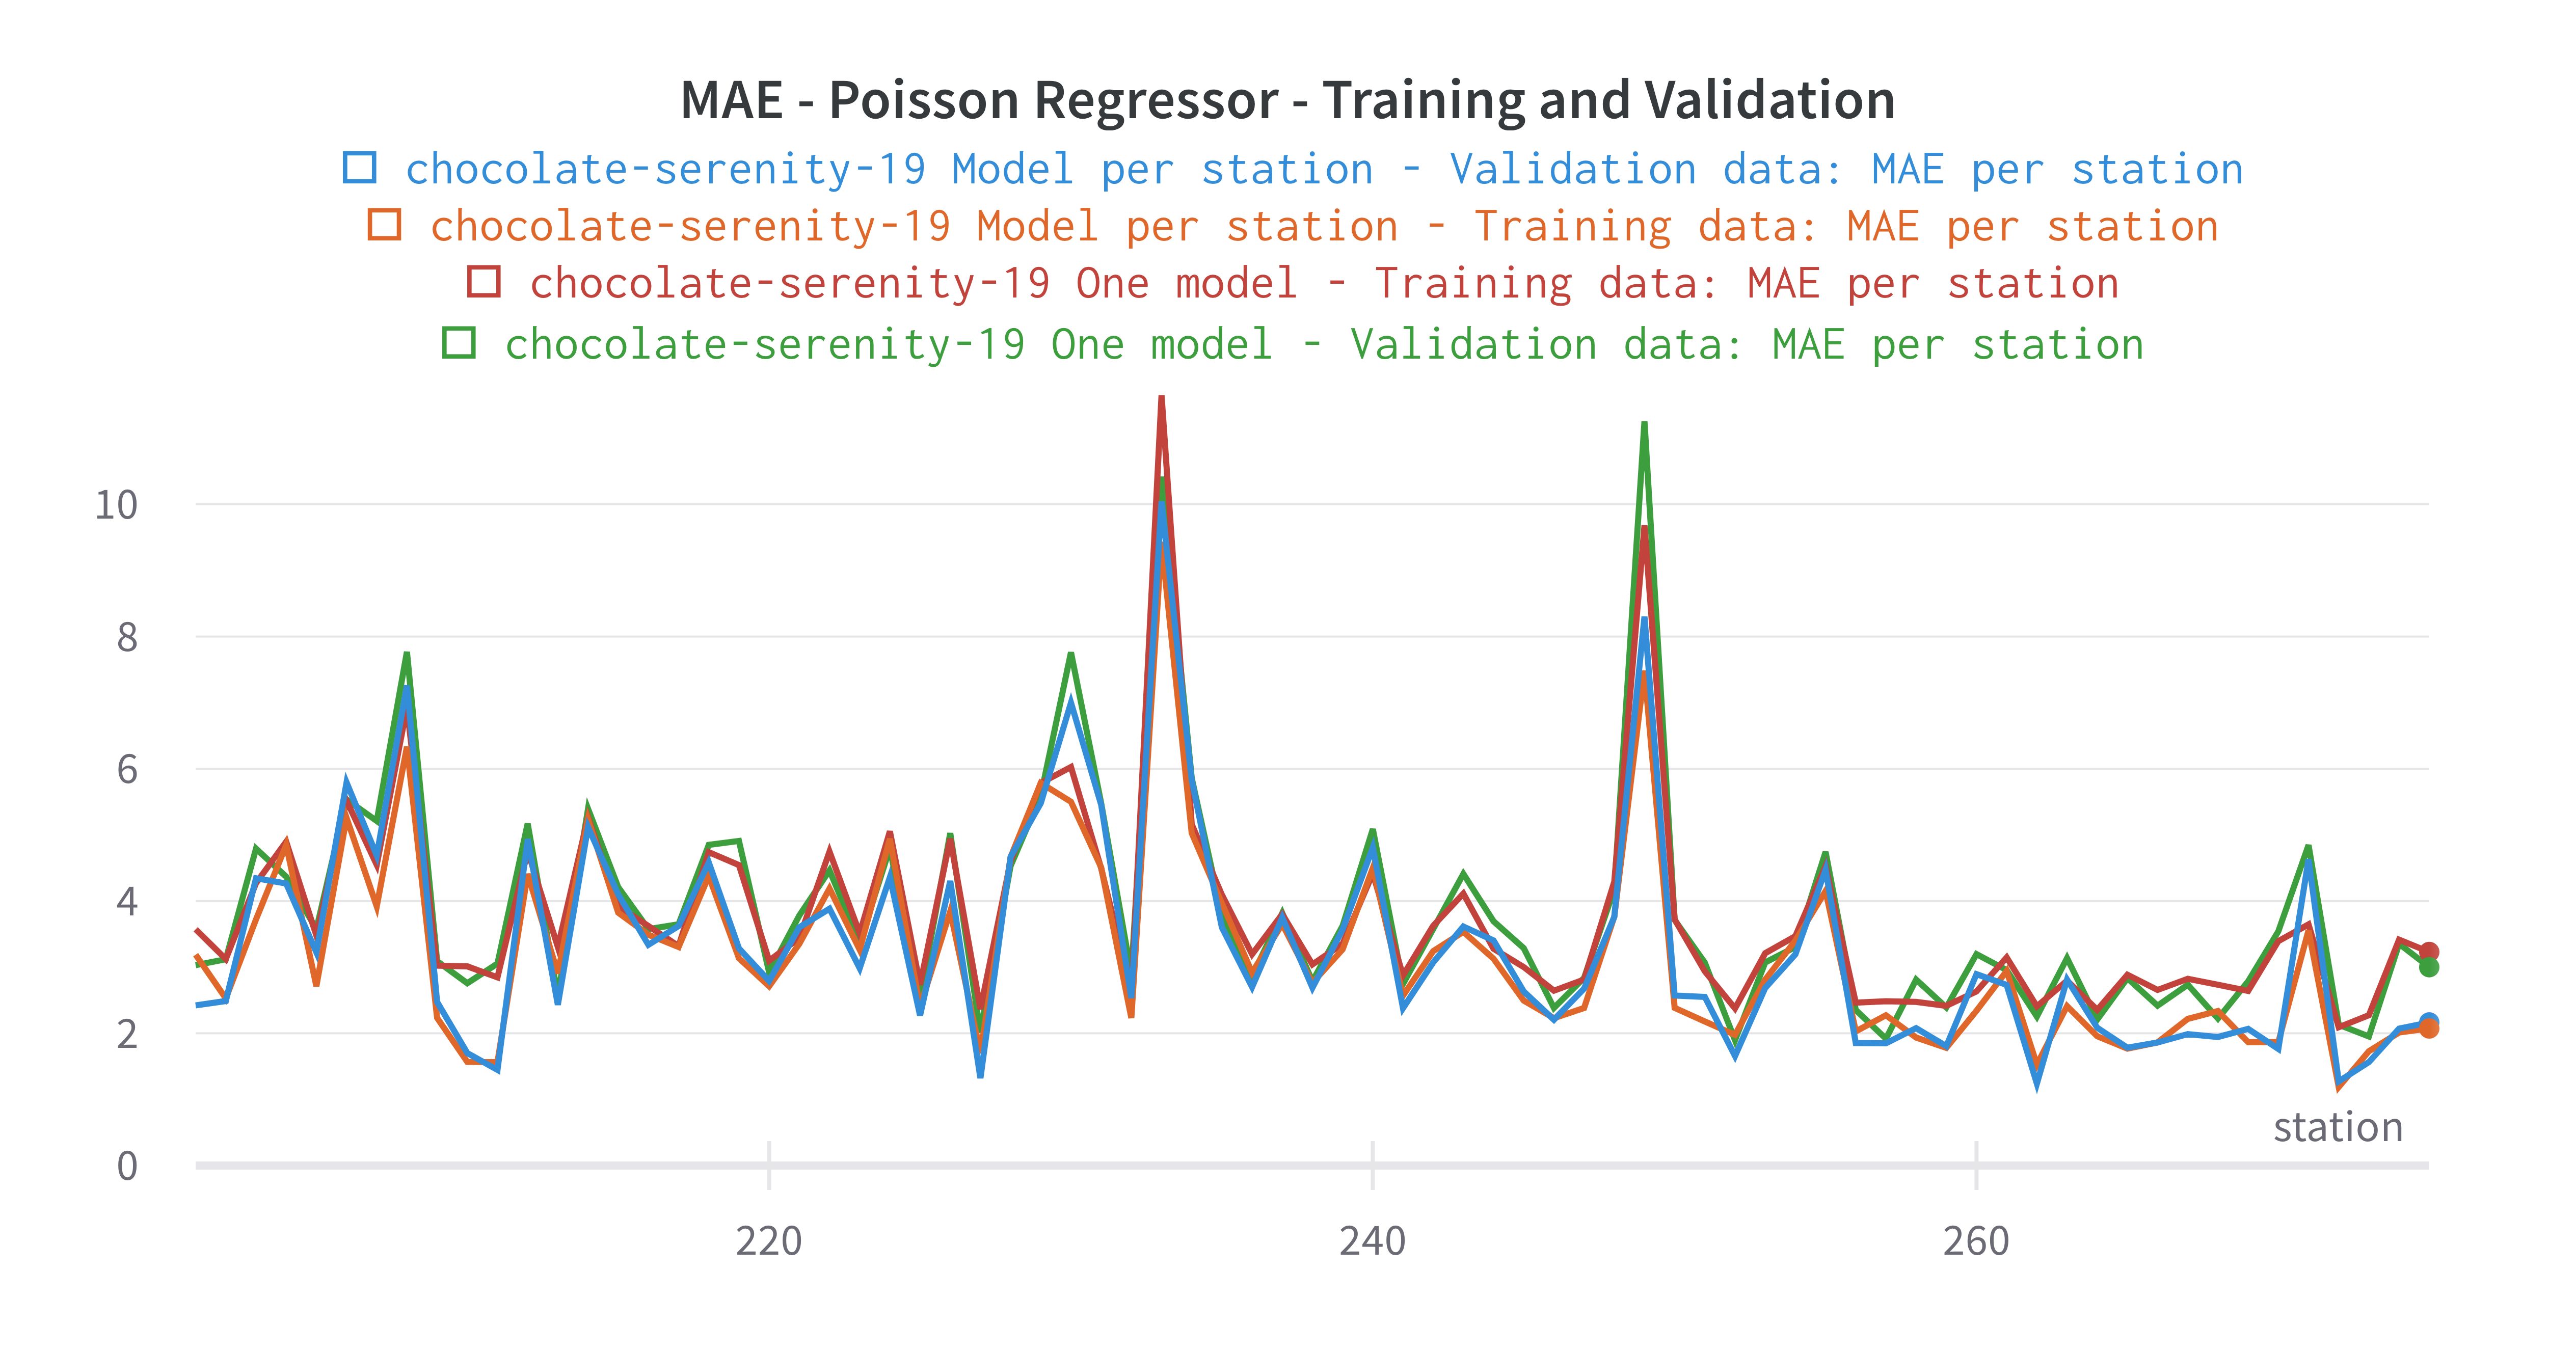
\includegraphics[width=0.5\textwidth]{mae-pr-perstation}\hfill
        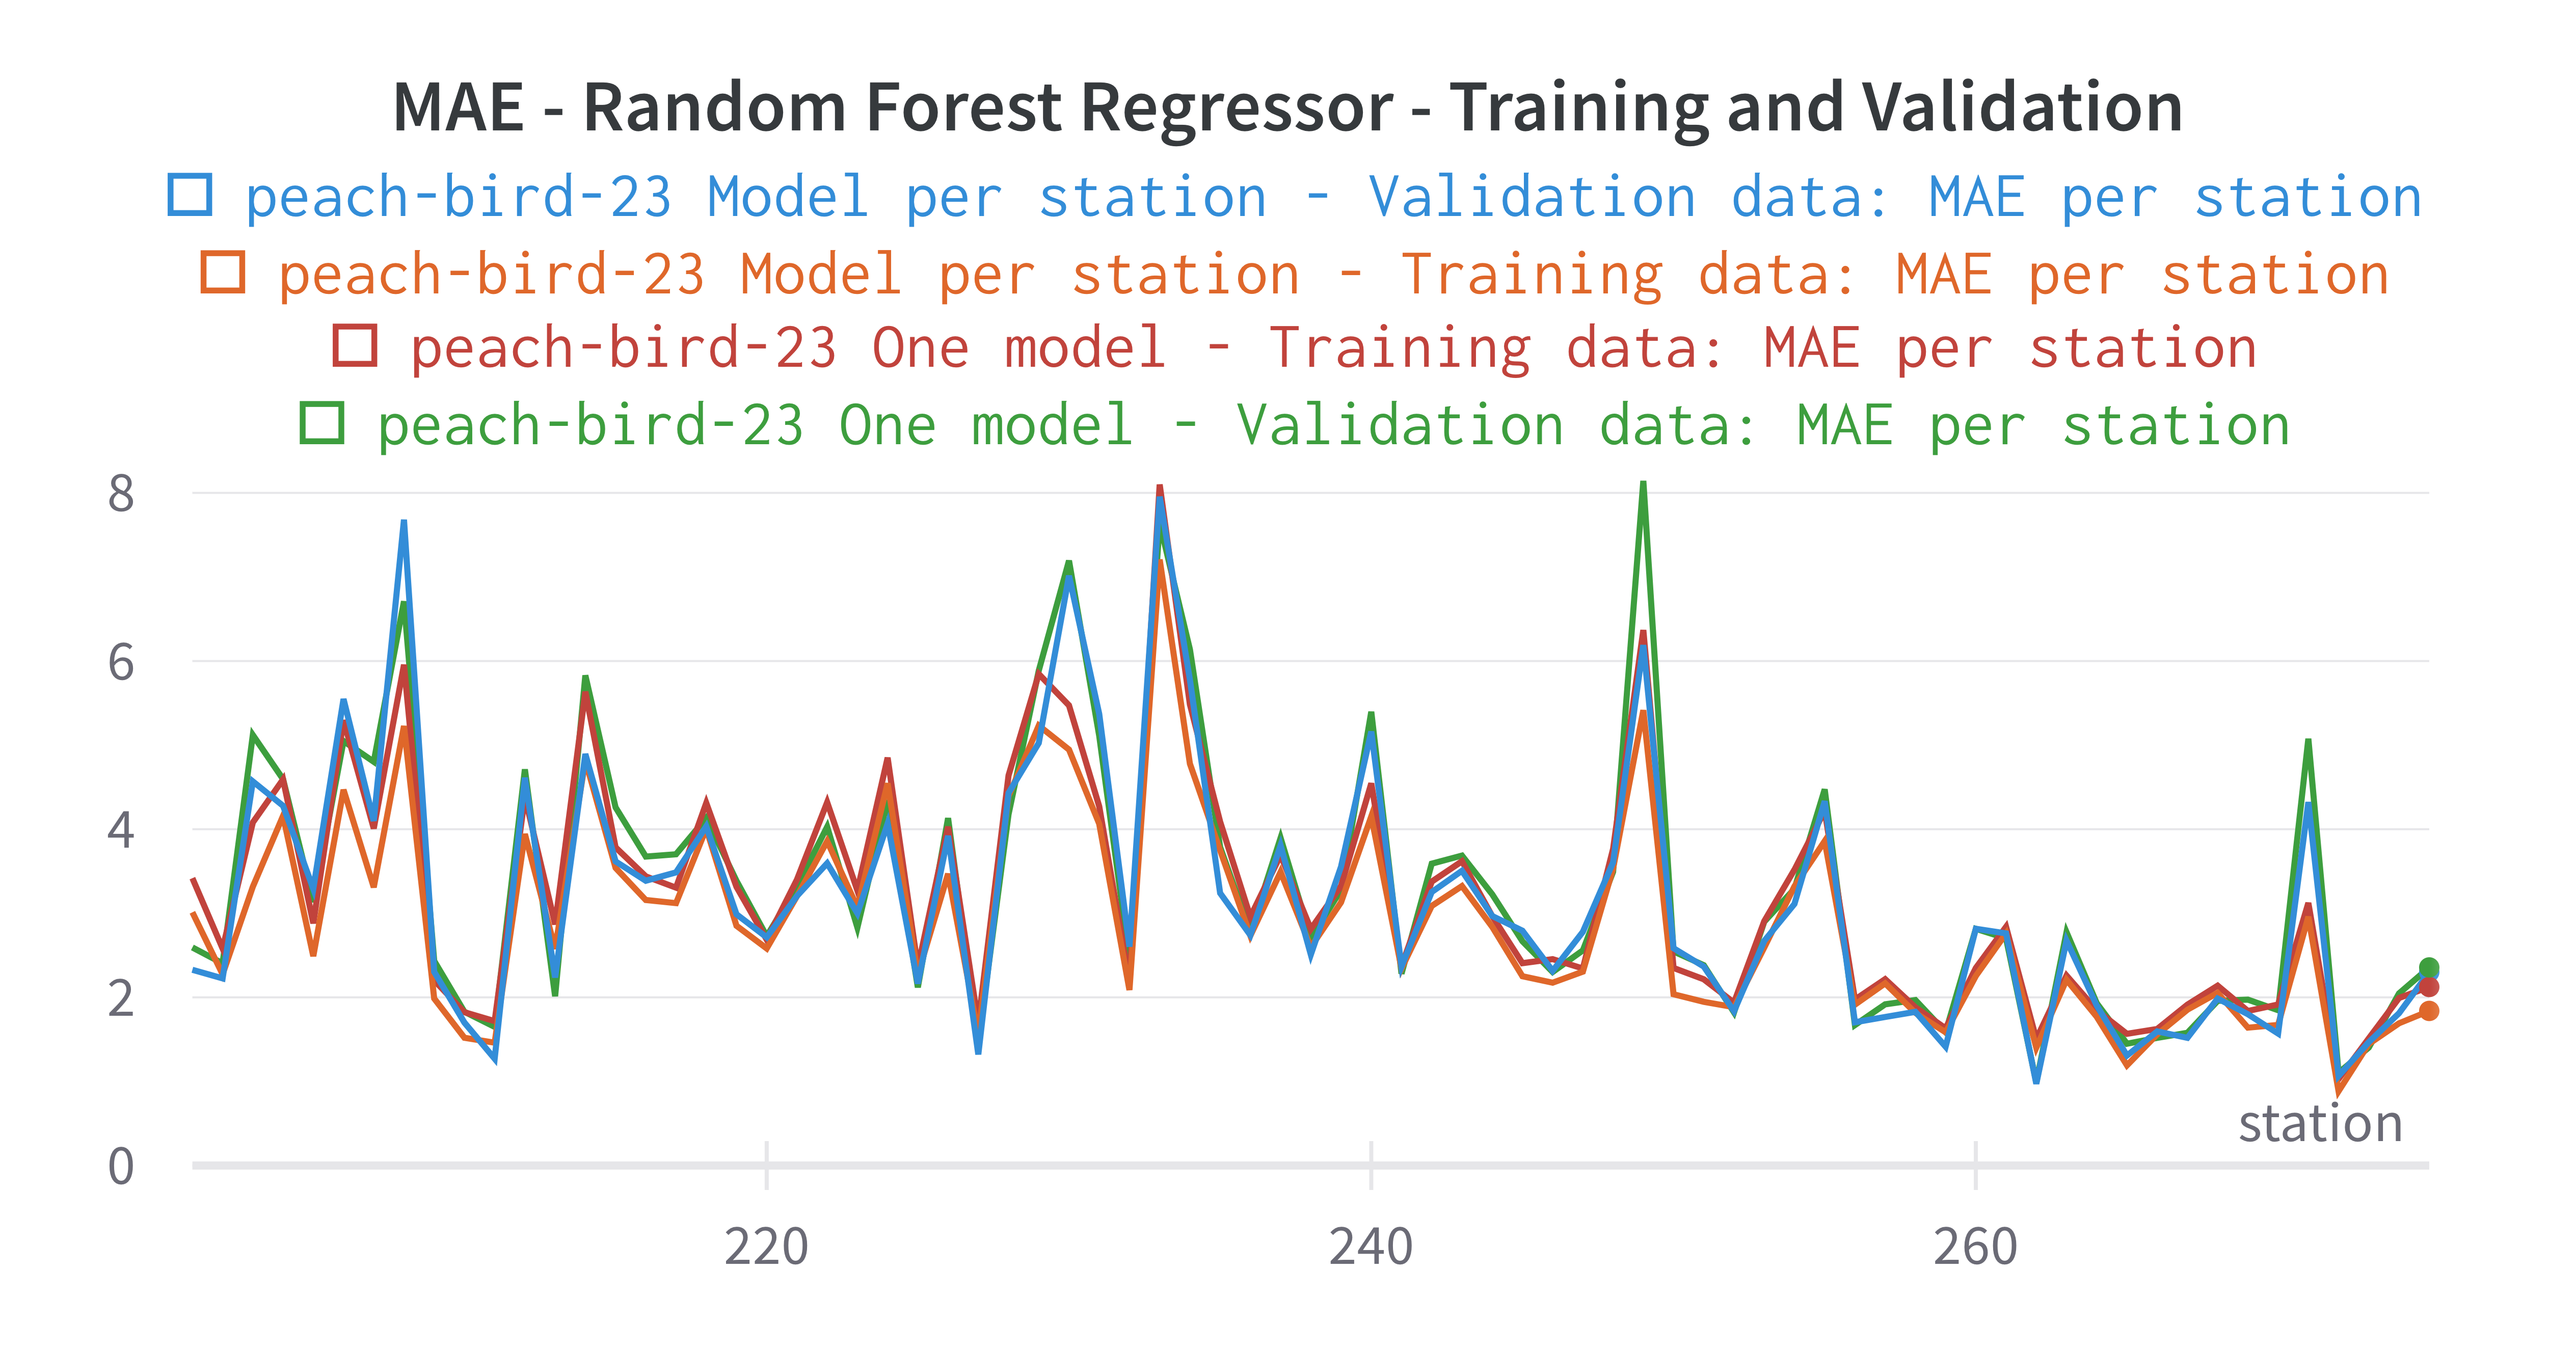
\includegraphics[width=0.5\textwidth]{mae-rfr-comparison}
        \caption{MAE per station for training and validation dataset for both both model per station and a single model}
        \label{fig:simple-pr-rfr-mae-perstation}
    \end{figure}


    Poisson:

    Features = Bikes\_3h\_ago \& num Docks
    One model - training data mae = 3.661
    One model - validation data mae = 3.706
    per station - training data mae = 3.236
    per station - validation data mae = 3.327

    -> Model per station performs slightly better with minimal additional time for the single model
    -> no difference in features used for model per station

    -> overall the model per station performed better

    Random Forest Regressor:
    First run: one feature 3h\_bikes - 4th peach-bird
    Model per station - Training data: MAE 2.90715
    Model per station - Validation data: MAE 3.14552
    One model - Training data: MAE 3.19787
    One model - Validation data: MAE 3.28136

    Second run: 2 features num of Docks and 3h\_bikes - 4th autumn-rain
    Model per station - Training data: MAE 2.90709
    Model per station - Validation data: MAE 3.14749
    One model - Training data: MAE 3.12366
    One model - Validation data: MAE 3.26918

    One Model:
    Station differences:
    -> Random Forest does better for all stations, so far all algorithms struggle with a few stations:
    - station 233 - MAE 11.6 for PoissonRegressor (2 features - classic pyramid - training), ~8 for Random Forest * both (particularly in training ata)
    - station 249 - MAE 11.25 Poisson (classic pyramid - validation), 8.1 Random Forest (Peach bird - validation),
    6.3 (Peach bird - training)
    - station 208 - MAE 7.7 Poissn classic pyramid validation, 6.71 Random Forest Peach bird - validation
    - station 230 - MAE 7.6 Poisson classic pyramid validation, 7.1 Random Forest (peach bird - validation)

    -> A few stations do better than average
    - station 209-211, 213, 227, 252, 256-259, 262, 265-270, 272-275 all have MAE around 2 for Random Forest

    Differences in Training and Validation:
    - Most stations do worse in validation as expected given the algorithm is trained on the training data, however for station
    233 this is not the case it does worse in training (11.6training, 10.4 validation poisson-classic pyramid),
    (8.1 training, 7.6 validation peach bird -  random forest)

    For multiple models these trends are the same (the numbers are slightly different)
    - Multiple models perform slightly better (see weave)

    \subsubsection*{\nameref{itm:phase1-step3}}
    Poisson \& Random Forest Use More features
    1. Station (as location data)
    wobbly-hill-run -> include station
    Model per station - Training data: MAE 2.90737
    Model per station - Validation data: MAE 3.14606
    One model - Training data: MAE 2.91782
    One model - Validation data: MAE 3.14946
    -> this had the wished effect that the difference between using a model per station and using just one model
    becomes way smaller
    -> However it does not necessarily hold true for the validation dataset

    2. Add Weekhour (as demand data based on weekday and time of day)
    Model per station - Training data: MAE 1.05213
    Model per station - Validation data: MAE 2.26165
    One model - Training data: MAE 1.18072
    One model - Validation data: MAE 2.52993

    -> this had a profound impact removing the significance of the peaks for the bad stations
    -> However it also increased the gap between training data and validation. The start of overfitting
    -> On 50\% of the test data this avhieve 2.92266

    3. Add weather data:vital-hill
    - Precipitation cannot be added as it is 0.0 for all the provided data so nothing can be learned form it
    alhtough it probably would be impactful
    Run Vital Hill -> it's overfitting and performs worse than the model without weather!
    Model per station - Training data: MAE 0.91045
    Model per station - Validation data: MAE 2.51165
    One model - Training data: MAE 1.10876
    One model - Validation data: MAE 2.8752

    4. Add is holiday: astra feather
    Model per station - Training data: MAE 1.00044
    Model per station - Validation data: MAE 2.21935
    One model - Training data: MAE 1.13664
    One model - Validation data: MAE 2.48154
    -> better than weather data

    5. Add air pressure back: driven cosmos - overfitting starts again
    Model per station - Training data: MAE 0.8418
    Model per station - Validation data: MAE 2.27939
    One model - Training data: MAE 1.04464
    One model - Validation data: MAE 2.67455


    6. Replace air pressure with temperature -> soft deluge
    Model per station - Training data: MAE 0.91617
    Model per station - Validation data: MAE 2.40878
    One model - Training data: MAE 1.09112
    One model - Validation data: MAE 2.73405
    -> as predicted this overfitts worse, temperature is not a good parameter

    7. Use full Bike profiles -> Dauntless wood
    Model per station - Training data: MAE 0.83188
    Model per station - Validation data: MAE 2.31577
    One model - Training data: MAE 0.92461
    One model - Validation data: MAE 2.419
    -> not as good as astral feather but not as overfitting as the weather!


    \subsubsection*{\nameref{itm:phase1-step4}}

    Random Forest Sweep 1:
    - Show most influential parameter
    - Show graphs
    Parameters:
    - random\_forest\_n\_estimators:  [50, 100, 120] \# made no difference
    - random\_forest\_criterion: ['squared\_error', 'absolute\_error']  \# squared\_error better than poisson, try absolute error
    - random\_forest\_max\_depth: [None, 10, 50]  \# 50 better than 100!
    - random\_forest\_min\_samples\_split: [2, 4] \# made no difference
    - random\_forest\_ccp\_alpha: [0.0, 0.05, 0.1, 0.3]  \# unclear but 0.05 did well
    -> criterion squared\_error speeds up the training significantly (not to sure yet how it impacts the performance)
    -> The difference in MAE between training and validation however was reduced, this did not impact the overal outcome though

    Silver Plasma: https://wandb.ai/idegen/mlp-2021/runs/1t2bcd2d/overview?workspace=user-idegen
    -> Best sweep result does not compete with default configurations

    Model per station - Training data: MAE 1.393
    Model per station - Validation data: MAE 2.72
    One model - Training data: MAE: 2.918
    One model - Validation data: MAE 2.947

    Breezy Sound: https://wandb.ai/idegen/mlp-2021/runs/12p54n9c/overview?workspace=user-idegen
    -> New parameters but features as current best run with default configuration

    Model per station - Training data: MAE 1.514
    Model per station - Validation data: MAE 2.432
    One model - Training data: MAE 3.273
    One model - Validation data: MAE 3.394

    Stoic Sun: https://wandb.ai/idegen/mlp-2021/runs/12zlftk6/overview?workspace=user-idegen
    -> Features from best run squared error and ccp from sweep, max depth and n estimator from best run (exactelly the same!?)
    Worse then astral feathers
    Model per station - Training data: MAE: 1.514
    Model per station - Validation data: MAE: 2.432
    One model - Training data: MAE: 3.273
    One model - Validation data: MAE: 3.394

    -> More sweeping with more data, model per station instead of one model, smaller ccp's

    Sweep 2:
    - ?
    -> decision try astral feather with ccp of 0.001
    -> Result is zesty field on per station only which is better
    Model per station - Training data: MAE 1.00787
    Model per station - Validation data: MAE 2.20771
    (good thread on the different parameters: https://stackoverflow.com/questions/20463281/how-do-i-solve-overfitting-in-random-forest-of-python-sklearn)

    Sweep 3:
    - Impurity did not result in better performance for the real dataset
    - also setting random to 0 makes the runs reproducible

    Sweep 4: Features and Hyperparmetes
    - Impurity in combination with more features create a better result which could be confimred with floral-pine
    Model per station - Training data: MAE 0.89522
    Model per station - Validation data: MAE 2.20609
    -> For the random forest model the features used in the given models do not perform as well

    \subsection*{\nameref{phs:two}}
    \subsubsection*{\nameref{itm:phase2-step1}} Analyse the given models
    \subsubsection*{\nameref{itm:phase2-step2}} Create an end to end pipeline for the given models
    \subsubsection*{\nameref{itm:phase2-step3}} Investigate the resulting performance and compare to \nameref{phs:one}

    \subsection*{\nameref{phs:three}}
    \subsubsection*{\nameref{itm:phase3-step1}} Create an end to end pipeline for the combining the models from \nameref{phs:one} and \nameref{phs:two}
    \subsubsection*{\nameref{itm:phase3-step2}} Tune promising setups
    \subsubsection*{\nameref{itm:phase3-step3}} Investigate the resulting performance and compare to \nameref{phs:one} and \nameref{phs:two}


    \section{Conclusions}\label{sec:conclusions}
    share any insights you gained about how the system works.

    \subsection*{\nameref{phs:one}}
    \subsubsection*{\nameref{itm:phase1-step1}}
    From the data given I decided that this problem was most naturally a multivariate regression problem where I had to
    predict for each hour of the day the number of bikes a the station. I could perhaps also use a classifier given that
    the number I had to predict was from a discrete set of numbers. It's a supervised learning problem given I have 55800
    in total respectively 744 per station labelled data samples. I could do more feature exploring with clustering to
    learn how the different features relate to each other. However, I decided to first build an end to end pipeline using
    just the bikes\_3h\_ago as feature and building the ability to easily change the model and features as well as their
    pre-processing used.

    \subsubsection*{\nameref{itm:phase1-step2}}
    The design for the codebase and wandb worked out much better than what I initially did for the Dialogue and Narrative
    course work. The configuration got quite big and messy in the end and will need a bit more thought to
    keep more seperated between different models and experiments. Furthermore for a bigger project it definitely would
    make sense to store the model and save it too, both for
    reproducibility as well as saving time. Most of the model I played with have some randomness injected that is
    beneficial to the model's performance but which makes it impossible to exactly reproduce an experiment. Furthermore
    keeping the data in memory only works for a small dataset like the one we've been given. For a bigger dataset I
    would need to avoid keeping all data in memory at all time and use a disk/database streaming solution.

    I was suprpised how well the Poisson Regressor worked. It was considerable faster than the Random Forest Regressor
    and depending on I could see it being good enough to be able to estimate bikes within an error of $\pm$4 bikes.
    Figure \ref{fig:simple-pr-rfr-mae-perstation} shows however that for some station the error is bigger
    than the overall MAE and the pattern between which stations do well and which stations do badly is the same between the
    two models. However, the error for these stations is smaller for the Random Forest Regressor.

    While I didn't wanted to make a call at this point on which approach is better, the per station model did consistently
    perform better.

    \subsubsection*{\nameref{itm:phase1-step3}}
    - not enough exprimentation with nan values and the impact of my decision
    - sweep earlier and for features too
    - don't humanise about features these alorithm see different patterns

    \section*{Acknowledgements}

    \bibliographystyle{plain}
    \bibliography{bibliography}
%TODO reference the varsious medium articles for software engineering
\end{document}
